\documentclass{sig-strict}
\usepackage{amssymb,amsfonts,amsmath}
\usepackage{url,graphicx,multirow,hyperref,color,calc,ulem,threeparttable,tabularx,tabulary,booktabs,enumitem,subcaption,balance}
\usepackage[group-separator={,}]{siunitx}

\hypersetup{
  bookmarks=true,
  unicode=true,
  pdftoolbar=true,
  pdfmenubar=true,
  pdffitwindow=true,
  pdfstartview={FitV},
  pdftitle={},
  pdfauthor={},
  pdfnewwindow=true,
  colorlinks=false,
  pdfdisplaydoctitle=true,
  pdfborder={0 0 0}
}
\usepackage[absolute]{textpos}

\setlength{\TPHorizModule}{1in}
\setlength{\TPVertModule}{1in}
\textblockorigin{1in}{1in}

\paperheight 11in
\paperwidth 8.5in

\usepackage[all]{hypcap}

\makeatletter
\renewcommand*{\@fnsymbol}[1]{\ensuremath{\ifcase#1\or ^{\dagger}\or \ddagger\or
   \mathsection\or \mathparagraph\or \|\or **\or \dagger\dagger
   \or \ddagger\ddagger \else\@ctrerr\fi}}
\makeatother
\newcommand*\samethanks[1][\value{footnote}]{\footnotemark[#1]}

\input{.xxxnote}
\input{.blue}
% 16 Nov 2010 : GWA : Any special macros or other stuff for this particular
%               paper go here.

\newcommand{\PhoneLab}{\textsc{PhoneLab}}
\hyphenation{Phone-Lab turn-around po-s-ters e-ven-ts pro-gramm-able test-bed}

\setlist{nolistsep}


\begin{document}
\conferenceinfo{SENSEMINE'13,} {November 14 2013, Roma, Italy.}
\CopyrightYear{2013}
\crdata{978-1-4503-2430-4/13/11}
\crurl{http://dx.doi.org/10.1145/2536714.2536718}
\copyrightetc{Copyright \the\copyrtyr\ ACM \the\acmcopyr\ ...\$15.00}

\permission{Permission to make digital or hard copies of all or part of this
work for personal or classroom use is granted without fee provided that
copies are not made or distributed for profit or commercial advantage and
that copies bear this notice and the full citation on the first page.
Copyrights for components of this work owned by others than ACM must be
honored. Abstracting with credit is permitted. To copy otherwise, or
republish, to post on servers or to redistribute to lists, requires prior
specific permission and/or a fee. Request permissions from
\href{mailto:Permissions@acm.org}{Permissions@acm.org}.}

\date{}

\title{\textsc{\LARGE PhoneLab}: A Large Programmable Smartphone Testbed}

\numberofauthors{1}

\author{
\alignauthor
Anandatirtha Nandugudi, Anudipa Maiti, Taeyeon Ki, Fatih Bulut\\
Murat Demirbas, Tevfik Kosar, Chunming Qiao, Steven Y. Ko and Geoffrey Challen\\[0.05in]
\affaddr{Department of Computer Science and Engineering}\\
\affaddr{University at Buffalo}\\[0.05in]
\email{\href{email:team@phone-lab.org}{team@phone-lab.org}}\\[0.02in]
\email{\href{http://www.phone-lab.org}{\Large \texttt{www.phone-lab.org}}}
}

\maketitle

\ifdefined\isblue
\begin{textblock}{1}(6.4,0)
\noindent\href{http://blue.cse.buffalo.edu}{
\includegraphics[width=0.6in]{./figures/logos/blue.jpg}}
\end{textblock}                                                                                
\fi

Although smartphones have emerged as the most significant large-scale mobile
platform in computing history, the scale of smartphone experimentation has
lagged behind. Keeping pace requires new facilities that enable
experimentation at scale to ensure that research discoveries translate to the
growing network of smartphone devices.

This paper introduces \PhoneLab{}, a 288-device smartphone testbed deployed
at SUNY Buffalo. \PhoneLab{} provides access to an incentivized group of
participants ready to engage in Android experimentation. The testbed will
open for public experimentation in October, 2013, and continually grow by 2014.

To demonstrate the power of \PhoneLab{} we present three selected results
from a usage characterization experiment run on 115 phones for 21
days~\XXXnote{GWA: Need to update these numbers.}. We use each result to
motivate a future \PhoneLab{} experiment, demonstrating the power of
\PhoneLab{} to enable mobile systems research.


\category{D.4}{Operating Systems}{Distributed systems}

\terms{Design, Experimentation, Measurement, Performance}

\keywords{Smartphones, testbed, mobile devices}

\section{Introduction}
\label{sec-introduction}

\sloppypar{Smartphones have become the most popular computing platform.
Google reports 1.3~M Android device activations per day in September,
2013~\cite{google-Sep2012-activations}, while IDC projects that 224~M
smartphone units will ship worldwide in 2013 Q4, a 40\% increase over 2012
Q4~\cite{idc-smartphone-growth}. Taken as a whole, the growing network of
smartphone devices represents the largest, most pervasive distributed system
in history.}

Meanwhile, the scale of smartphone experimentation is not keeping pace. A
small survey of MobiSys'12 papers~\XXXnote{GWA: Could expand this to
MobiSys'13 or SenSys'13.} reveals that when smartphone evaluations use real
devices, they use small numbers of phones---3, 12, or
20~\cite{nowar-mobisys12,comon-mobisys12,caching-mobisys12}. Other
experiments use simulations driven by small, old, or synthesized data
sets~\cite{falcon-mobisys12,ace-mobisys12,humanmobility-mobisys12}. In either
case, large-scale results from real users would be more compelling. While
multiple factors---including recruitment, human subjects compliance, and data
collection---make large-scale smartphone experimentation challenging,
harnessing the growth of smartphones requires evaluating new ideas at scale.

\PhoneLab{} provides the features necessary for smartphone research---power,
scale, realism, locality, and relevance:

\begin{itemize}[nosep,leftmargin=*]
\vspace*{0.08in}
\item {\bf Scale:} \PhoneLab{} will grow to 700 participants, already
recruited to participate in experiments.
\item {\bf Power:} \PhoneLab{} allows application-level experiments as well
as platform-level, i.e., Android kernel, middleware, libraries, and Dalvik
virtual machine.
\item {\bf Realism:} Participants use the phones as their primary device.
\item {\bf Locality:} Most participants live in Buffalo near SUNY campuses,
enabling research requiring device-to-device interaction.
\item {\bf Relevance:} \PhoneLab{} allows researchers to stop relying on
out-of-date datasets. Instead, new data can be collected in the most
appropriate way for the experiment.
\vspace*{0.08in}
\end{itemize}

We present \PhoneLab{}, a large programmable smartphone testbed providing all
of these features together and enabling smartphone research at scales
currently impractical. \PhoneLab{} provides access to a large and stable set
of participants incentivized to participate in smartphone experimentation.
With 191~participants in 2012, and \XXXnote{XXX} in 2013, \PhoneLab{} will
grow to over 700~\XXXnote{GWA: Alter.} participants in 2014. By exploiting
locality, \PhoneLab{} increases the density and interaction rate between
participants, facilitating the evaluation of phone-to-phone protocols and
crowd-sourcing algorithms.~\XXXnote{GWA: Drum up the sensing aspects?}

By utilizing the Android open-source smartphone platform, \PhoneLab{} enables
research above and below the platform interface. Researchers can distribute
new interactive applications or non-interactive data loggers, but can also
change core Android platform components, allowing \PhoneLab{} to host systems
experiments impossible to distribute through the Play Store.

We make two contributions in this paper. First, we introduce \PhoneLab{}.
Section~\ref{sec-testbed} describes the testbed design and implementation,
and the Android logging framework and the visibility it provides into the
Android platform. Second, we demonstrate that \PhoneLab{} is powerful and
usable. Section~\ref{sec-experiment} describes a usage measurement experiment
run by 115 \PhoneLab{} participants for 21 days~\XXXnote{GWA: FIXME.}. Rather
than attempting a comprehensive analysis of the dataset, we use it to
highlight the power of \PhoneLab{} and breadth of research it supports. To do
so, Section~\ref{sec-usage} presents three results on:

\begin{itemize}
\item opportunistic charging (Section~\ref{subsec-opportunistic}),
\item 3G to Wifi transitions (Section~\ref{subsec-networktransitions}),
\item location data sharing (Section~\ref{subsec-locationsharing}).
\end{itemize}

For each, we first present our data and then describe how to use \PhoneLab{}
to perform further investigation. We hope that these examples will encourage
\PhoneLab{} use by the mobile systems community.

\section{The PhoneLab Testbed}
\label{sec-testbed}

\PhoneLab{} began operating in 2012 with 191~participants\footnote{We refer
to people carrying \PhoneLab{} phones and participating in experiments as
\PhoneLab{} \textit{participants}, to differentiate them from researchers
running \PhoneLab{} experiments which we call \textit{users}.} using
Nexus~S~4G smartphones~\cite{nexuss4g} running Android
4.1.1~\cite{jellybean}. The first year of operating was a beta test allowing
us to develop the software and expertise necessary to manage a large testbed.
No external experiments were solicited, but several internal experiments were
performed including a usage characterization study that produced the results
described in Section~\ref{sec-experiments}. In 2013, \PhoneLab{} grew to
288~participants using Samsung Galaxy~Nexus devices~\cite{nexuss4g} running
Android 4.2.2. Participants receive discounted voice, data, and messaging
from Sprint in exchange for their participation, and are required to use
their \PhoneLab{} phone as their primary device.

\PhoneLab{} experiments are either distributed through the Play Store or as
platform over-the-air (OTA) updates. Participants are notified of new
experiments and choose whether to participate after reviewing what
information will be collected about them. \PhoneLab{} participants are
\textit{required} to participate in experimentation but \textit{not required}
to participate in any particular experiment. They may remove experiments that
they deem too intrusive or that negatively affect their device. Some
experiments may run in the foreground and interact with users like typical
applications, while others may gather data silently in the background.

\PhoneLab{} users must provide human subjects review documentation, a list of
log tags to capture (which we describe later in this section), and their
experimental software---either a link to the Play Store or a patch against
the current \PhoneLab{} platform source.  Experiments generate data through
the standard Android logging interface. Log messages generated by \PhoneLab{}
experiments are captured and uploaded to a central server while the device is
plugged in and charging. When experimentation completes, the user receives an
archive containing every log message matching their tags generated by all
participating devices.

\subsection{Platform and Device}

\PhoneLab{} phones run the popular Google Android Open-source Smartphone
Platform (AOSP). Using an open-source platform for \PhoneLab{} was an obvious
choice for obvious and less-obvious reasons. The obvious reason is that the
AOSP allows \PhoneLab{} users to experiment with any software component,
meeting our goal of providing a powerful testbed. Modifications to Android
services that provide location, access networks, and manage power can be
benchmarked alongside unmodified devices. Of course, power also creates
problems: faulty experiments can render phones inoperable and threaten
participation. As a result, experimentation at the platform level will
require additional pre-deployment testing and interaction with the
\PhoneLab{} team when compared with experiments that only distribute novel
applications or collect data at the application level. We plan to begin
supporting external platform experimentation in 2014.

We have also found that using an open-source platform has other, less obvious
benefits. First, the availability of the Android source makes \PhoneLab{}
instrumentation easier even when collecting data from the application level
because it gives a visibility into hidden APIs. For example, our usage
characterization experiment, described in Section~\ref{sec-experiments}, uses
Java reflection to access hidden battery usage APIs. Second, using the AOSP
allows us to sign the platform image used by our participants. When the same
key is used to sign a software package, that application may run as the
system user with root privileges. Using this feature allows us to distribute
and update core \PhoneLab{} experimental management software via the Play
Store while retaining the privileges necessary to collect logs and perform
platform updates.

Finally, we expect that our base \PhoneLab{} platform image will evolve to
meet the needs of the research community. While we have found that Android
already logs a wealth of information about platform operation, there are
places where more information could be exposed or logged in a more
experiment-friendly way. Controlling the platform provides the opportunity to
supplement existing interfaces or add additional logging to facilitate
experimentation.

We distributed Samsung Nexus~S~4G smartphones to our first year of
participants and Samsung Galaxy~Nexus smartphones to our second year. Both
were official AOSP development phones and are well-supported, although we had
to obtain proprietary drivers directly from Sprint for the Galaxy~Nexus.
While we expect to receive yearly phone upgrades and will distribute a more
up-to-date device to our second group of participants, we anticipate that the
prohibitive cost of the newest flagship smartphones will prevent us from ever
deploying them on \PhoneLab{}.

\subsection{Participants}

\XXXnote{GWA: TODO: Maulik}

Recruiting a large number of \PhoneLab{} participants requires effective
incentives. In their first year of \PhoneLab{} participation, voice, data and
messaging are free with funding provided by the National Science Foundation
(NSF). This free year of service plays a major role in our recruiting
efforts. In subsequent years, participants pay a deeply discounted \$45 per
month rate for unlimited data and messaging through a deal negotiated with
Sprint. Sprint has proved to be an ideal partner for the \PhoneLab{} project,
both helpful with testbed logistics and still willing to provide unlimited
data plans to subscribers.

Because participants may leave at any time, the front-loaded cost structure
of our incentives makes it most efficient to recruit participants who will be
able to continue as part of \PhoneLab{} for multiple years. While we
anticipate that some of our first group of participants will leave after a
single year, interviews with them will help us identify long-term
participants during subsequent years. Long-term participants allow us to
amortize the first free year and provide a stable group comfortable being a
part of \PhoneLab{} experimentation.

When recruiting our first batch of participants (Year 2012-2013), we targeted freshman
and sophomore SUNY Buffalo (UB) students as well as incoming PhD students. The
University at Buffalo has a large international graduate student community, and
many of these students arrive on campus without phones or phone contracts,
making them ideal multi-year \PhoneLab{} participants. After a first round of
smartphone distribution in late August and early September 2012, we also began
to reach out to the professional population at SUNY Buffalo in an effort to
increase the number of potential long-term participants as well as the diversity
of our participant pool.

For recruiting our second batch of participants (Year 2013-2014), we targeted mostly 
SUNY Buffalo (UB) PhD students and Staff/faculty members with focus on getting potential 
multi-year \PhoneLab{} participants. This has also added the diversity to our overall participant pool demographics.

\begin{table*}[t]
  \begin{subtable}[t]{\columnwidth}
    \begin{tabularx}{\columnwidth}{Xr@{\hspace{0.5in}}Xr}
    \multicolumn{4}{c}{\textbf{Gender}} \\
    \midrule
    Female & 51 & Male & 140 \\[0.1in]
    \multicolumn{4}{c}{\textbf{Age}} \\
    \midrule
    Under 18 & 12 & 30--34 & 15 \\
    18--19 & 74 & 35--39 & 6 \\
    20--21 & 12 & 40--49 & 13 \\
    22--24 & 22 & 50--59 & 7 \\
    25--29 & 29 & 60+ & 1 \\
    \end{tabularx}
    \caption{\textbf{2012--2013}, 191 participants.}
  \end{subtable}
  \begin{subtable}[t]{\columnwidth}
    \begin{tabularx}{\columnwidth}{Xr@{\hspace{0.5in}}Xr}
    \multicolumn{4}{c}{\textbf{Gender}} \\
    \midrule
    Female & 127 & Male & 122 \\[0.1in]
    \multicolumn{4}{c}{\textbf{Age}} \\
    \midrule
    Under 18 & 0 & 31--35 & 35 \\
    18--20 & 12 & 36--40 & 28 \\
    21--24 & 21 & 41--50 & 52 \\
    25--26 & 19 & 51--60 & 34 \\
    27--30 & 34 & 60+ & 9 \\
    \end{tabularx}
    \caption{\textbf{2013--2014}, 288 participants.}
  \end{subtable}
\caption{\textbf{Demographic breakdown of \PhoneLab{} participants.} Date
ranges are inclusive.}
\label{table-demographics}
\end{table*}



In the end, we believe that we were successful in recruiting potential
long-term participants. Table~\ref{table-demographics} describes the
demographic breakdown that we achieved. We have handed out our phones to
several masters or senior students because they are involved \PhoneLab{}
research. The majority consists of potential long-term participants. 
For first year, roughly half of our participants were first- and second-year undergraduates, 
a quarter PhD students, and a fifth faculty, staff and other professionals. Males greatly outnumber females, 
and the young outnumber the middle-aged and older.  
We rectified unrepresentative features in second year. We have achieved equal male and female participants
and middle-aged/older participants outnumber the younger participants. 
For management reasons we limited participation to people with a SUNY Buffalo
affiliation.

\subsection{Testbed Software}

\PhoneLab{} devices are deployed with a small piece of testbed management
software embedded in the Android platform image. This heartbeat service
uploads periodic reports including information about device location, battery
levels, and the installation status of other core \PhoneLab{} components.
This information is only used for testbed management and will never be
released to researchers.

The heartbeat service is also responsible for starting the primary
\PhoneLab{} configuration and data collection software when the phone boots,
which allows us to bypass an Android security feature that normally prevents
services from running in the background unless started by a foreground
application. In order to remain unobtrusive, our experimental management
software does not have a foreground component and thus would not normally be
able to start.

Experimental configuration, log collection, data upload and platform updates
are performed by the \PhoneLab{} experimental harness, which is installed and
updated through the Google Play Store. By signing it to match the platform
build key it runs with root privileges, necessary to collect logs from all
applications and perform platform updates. Periodically, the experimental
harness retrieves an XML configuration from a central \PhoneLab{} server. The
configuration specifies what background experiments to start or stop, what
data to collect, which server the phone should upload data to and the policy
for when to perform uploads. The \PhoneLab{} harness also uploads status
information to the server during the configuration exchange, including what
versions of various harness components are installed, what experiments are
running and how much data is waiting to be uploaded.

\PhoneLab{} logging and data collection must be unintrusive. If it is not,
either our participants will leave or their usage patterns will be affected.
We believe that we have achieved this goal. First, measured battery usage of
\PhoneLab{} is low. A conservative overhead estimate that includes all of the
applications that run as the shared system user comes to a per-participant
average of 2.4\%. This should be considered a strict maximum. Our policy of
only uploading while the device is plugged and charging eliminates the
overhead of the most power-hungry task.

Second, we have received no major complaints about our the final version of
our \PhoneLab{} experimental harness after we instructed participants to
install it. Given that participants we allowed to use their phone without our
software for several months, we believe that any significant changes in phone
behavior caused by our experimental harness would have been noticed.

\subsection{Safety and Privacy}

\PhoneLab{} is different from many other computer systems testbeds, such as
Emulab~\cite{white:osdi:2002, emulab}, PlanetLab~\cite{peterson:ccr:2003,
planetlab}, MoteLab~\cite{werner-allen:ipsn:2005}, or
OpenCirrus~\cite{avetisyan:computer:2010, opencirrus}: our experiments
involve real people. There are two core requirements regarding our
participants. First, they should use their phone as they normally would,
which motivated the design of unintrusive testbed management software.
Second, and more importantly, they must feel safe and in control while part
of \PhoneLab{}.

To accomplish this, when possible, we leverage several existing safety
mechanisms. First, we require an Institutional Review Board (IRB) to review
each \PhoneLab{} experiment for human subjects compliance. IRB approval or an
official waiver is required before any \PhoneLab{} any experiment can begin.

Second, we distribute experimental applications to a group of developers
prior to broader release, allowing us to identify any significant problems
before they reach our participants. This step is particularly important for
platform experiments, which must be established as stable before being
distributed.

Finally, we utilize Android's existing safety and privacy mechanisms.
Participants are presented with the typical Android privacy dialog during
experiment installation. Rather than building an alternate distribution
channel or privacy mechanism, we felt it was sufficient and probably better
to use a process participants are familiar with. After installation, if a
participant discovers that an experiment malfunctions or wastes power, they
can uninstall it. If we notice patterns of experimental removal, we will flag
the experiment and notify the researcher.

\begin{table}[t]

\begin{tabularx}{\columnwidth}{Xrr}
\multicolumn{1}{c}{\normalsize{\textbf{Tag Name}}} & 
\multicolumn{1}{c}{\normalsize{\textbf{Tag Count}}} & 
\multicolumn{1}{c}{\normalsize{\textbf{\%}}} \\
\toprule
\texttt{ActivityManager} & \num{96251731} & 13.7 \\
\texttt{dalvikvm} & \num{92565828} & 13.1 \\
\texttt{ConnectivityService} & \num{19195475} & 2.7 \\
\texttt{ActivityThread} & \num{17447815} & 2.5 \\
\texttt{PhoneStatusBar} & \num{13823998} & 2.0 \\
\texttt{SizeAdaptiveLayout} & \num{9857534} & 1.4 \\
\texttt{wpa\_supplicant} & \num{9279597} & 1.3 \\
\texttt{System.err} & \num{8141399} & 1.2 \\
\texttt{SAN\_SERVICE} & \num{7530577} & 1.1 \\
\texttt{LocationManagerService} & \num{6640001} & 0.9 \\
\texttt{DexLibLoader} & \num{5438086} & 0.8 \\
\texttt{SecCamera} & \num{5436968} & 0.8 \\
\texttt{HeartbeatService} & \num{4871085} & 0.7 \\
\texttt{Beautiful Widgets(4120000)} & \num{4692578} & 0.7 \\
\texttt{AudioCache} & \num{4447544} & 0.6 \\
\texttt{k9} & \num{4330848} & 0.6 \\
\texttt{SensorActivatorService} & \num{4177370} & 0.6 \\
\texttt{ThrottleService} & \num{4121301} & 0.6 \\
\texttt{VoldCmdListener} & \num{4014302} & 0.6 \\
\texttt{WindowManager} & \num{3948168} & 0.6 \\
\texttt{AudioHardware} & \num{3913724} & 0.6 \\
\end{tabularx}

\caption{\textbf{Top 20 log tags generated by Android.} During 21~days
\PhoneLab{} collected \num{704216410} log messages from \num{7556} tags.}

\label{table-logtags}

\vspace*{-0.1in}
\end{table}


\begin{table*}[t]

\begin{tabularx}{\textwidth}{rrrX}
\multicolumn{1}{c}{\normalsize{\textbf{Tag Name}}} & 
\multicolumn{1}{c}{\normalsize{\textbf{Tag Count}}} & 
\multicolumn{1}{c}{\normalsize{\textbf{\%}}} & 
\multicolumn{1}{c}{\normalsize{\textbf{Description}}} \\
\toprule
\texttt{PhoneLabSystemAnalysis-Snapshot} & \num{4507143} & 71.8 & Collects battery breakdown across components and applications. Polled every 15 minutes. \\
\texttt{ActivityManager} & \num{1078872} & 17.2 & Logs application management actions. \\
\texttt{PhoneLabSystemAnalysis-Telephony} & \num{240882} & 3.8 & Records phone call state and radio signal strength. \\
\texttt{PhoneLabSystemAnalysis-BatteryChange} & \num{212929} & 3.4 & Logs every change to the battery level. \\
\texttt{PhoneLabSystemAnalysis-Wifi} & \num{144163} & 2.3 & Logs connection state, scan information and signal strength. \\
\texttt{LocationManagerService} & \num{45478} & 0.7 & Records when GPS is enabled and disabled. \\
\texttt{PhoneLabSystemAnalysis-Location} & \num{26588} & 0.4 & Passively logs all location updates. \\
\texttt{PhoneLabSystemAnalysis-Misc} & \num{20960} & 0.3 & Logs when the screen turns on and off. \\
\texttt{SmsReceiverService} & \num{2686} & 0.0 & Used to count text messages sent and received. \\
\texttt{PhoneLabSystemAnalysis-Packages} & \num{112} & 0.0 & Records when
applications are installed and removed. \\
\end{tabularx}

\caption{\textbf{Log tag statistics for one day during our
experiment.} \num{6279813} total log tags were collected.}

\label{table-experimenttags}

\end{table*}


\subsection{Experimental Procedures}

To conclude, we review \PhoneLab{} experimentation from a researcher's
perspective.

First, develop your application locally. Any information logged through the
standard Android logging library can be recorded. In addition, the platform may
already be logging useful information for you. Keep track of all the log tags
you want \PhoneLab{} to capture. Approach your local IRB and receive
experimental approval and upload your application to the Play Store.

Second, upload your list of log tags, IRB letter, and link to your
application on the Play Store through the \PhoneLab{} website. We will
contact you when we begin beta testing and again once your experiment is
ready for the testbed. During beta testing you will be provided with
\PhoneLab{} log output to ensure that your experiment is running properly.

Finally, your experiment will be scheduled. Our goal is to maintain a
medium-sized list of active experiments for our participants: large enough to
make good use of the testbed, but small enough to ensure that each experiment
is picked up by many participants. When your experiment completes, you will
receive a archive with messages matching the tags you selected.

\section{Example Experiments}
\label{sec-experiments}

During our first beta test year we performed a usage measurement study. 115
participants joined the study which ran for over six months. For this
purpose, we developed a measurement application that collects multiple
salient features of smartphone usage: networking, mobility, power
consumption, and application usage. This section presents selected results on
energy usage, wireless network transitions, and battery charging behavior.
Our goal is to demonstrate the types of experiments that can be performed on
\PhoneLab{} and the insights they can achieve.

\subsection{Energy Breakdown}
\label{subsec-energybreakdown}

A single-day component-by-component breakdown is shown in
Figure~\ref{figure-batteryoverview}. Our results are similar to those reported
by a previous smaller-scale study~\cite{shye:micro:2009}, and indicate that
mobile data (labeled as ``Idle data'' and ``Active data'' depending on the
state), the screen, and CPU usage are the main sources of power consumption. The
per-participant bars also show a great deal of variation, with differences in
both the amount and the breakdown of energy consumed by each participant.

One supposedly power-hungry component that has less of an impact than we had
expected is the GPS. This is particularly surprising given the large amount
of location-monitoring work motivated by GPS power consumption. One of
several factors may be at work. First, the Android platform estimates the GPS
chipset current consumption at 50~mA. This number is used by the standard
``Fuel Gauge'' battery monitor and by our calculations. However, it is lower
than the data sheet for the Broadcom 4751 GPS receiver~\cite{bcm4751} and may
represent a best-case average. Still, even if the GPS current consumption is
off by as much as a factor of five, it does not represent a significant
contribution. Other hypotheses are that Android network location is providing
location with sufficient accuracy for many applications, eliminating the need
for GPS, or participants and applications may simply be conscious of GPS
power consumption and taking steps to control it.

\begin{figure}[htb!]

\centering
\includegraphics[width=0.65\columnwidth]{./figures/power/opportunistic_charging/count_and_by_time/graph.pdf}

\vspace*{-0.1in}

\caption{\textbf{Charging patterns.} Many users perform opportunistic
charging during the day, with habitual charging occurring at night.}

\label{fig-opportunistic-patterns}

\vspace*{0.1in}

\centering
\includegraphics[width=\columnwidth]{./figures/power/opportunistic_charging/max_difference/graph.pdf}

\caption{\textbf{Charge difference between participants during one day.} The
graph plots the top and bottom quartiles as well as the median. At any given
time, a significant spread is present.}

\label{fig-opportunistic-spread}

\vspace*{-0.1in}

\end{figure}

\subsection{Opportunistic Charging}
\label{subsec-opportunistic}

One way that users work around the battery limitations of their smartphone
devices is by finding new times and places to charge their phones: plugging
in at their desk at work, in the car during their commute, or at home before
a long night out. We refer to these charging sessions as
\textit{opportunistic} to distinguish them from \textit{habitual} nightly
charging. Assuming that many smartphone users encounter plug points
throughout the day, engaging in opportunistic charging becomes an additional
sign of energy awareness, and understanding opportunistic charging becomes
necessary to improving energy management on mobile devices. Others have analyzed
this behavior before~\cite{banerjee:ubicomp:2007} and
our goal is to examine the battery charging behavior of \PhoneLab{} participants.

Figure~\ref{fig-opportunistic-patterns} shows that many users engage in
opportunistic charging. We define a charging session as opportunistic if is
longer than 10~minutes but does not restore the battery to a fully-charged
state, indicating that the user disconnected the device before charging could
finish. On a representative day during our experiment, of the 245 charging
sessions we observed that day, 96 (39\%) were opportunistic by this
definition. 50 of 95 active participants engaged in opportunistic charging at
some point during our experiment an average of once per day.

Opportunistic charging may be a response to an anticipated need for more
smartphone battery power, as when a student plugs her smartphone in to charge
before a night out. Our data also allowed us to examine how many of these
opportunistic charging sessions were necessary to bridge the gap to the next
full charge. We found that 24 of the 96 (25\%) of the opportunistic charges
we observed were necessary. We believe that this indicates that participants
have responded to their smartphones' battery limitations by engaging in
conservative charging behavior, grabbing power whenever possible even if they
do not anticipate needing it later.

Opportunistic charging combined with the varied rhythms of our participants
creates a second interesting effect: at any given point there is a wide
disparity in the amount of power available on different phones.
Figure~\ref{fig-opportunistic-spread} displays the top, bottom, and middle
(median) quartiles for a single day on \PhoneLab{}. Only phones that are
discharging are shown, which explains the sharp increase between 6~and~10AM
as participants end nightly charging cycles.  As the graph indicates, it is
likely that when two smartphones meet they have very different battery
levels.

\subsection{Mobile Network Transitions}
\label{subsec-networktransitions}

Mobile smartphones move through a complex network environment. Providing the
illusion of seamless connectivity requires negotiating hand-offs both between
Wifi access points and between Wifi and 3G radios. We were interested in
observing hand-offs between 3G (provided by Sprint, \PhoneLab{}'s operational
partner) and Wifi and found many in the dataset collected by our usage
experiment. Since the Android \texttt{ConnectivityService} frequently
switches network interfaces for exploration purposes, we have defined a
transition as two one-minute or longer sessions on different interfaces
separated by less than one minute. We further limit ourselves to cases where
we received a location update during the transition. Data for the first
21~days of the usage experiment is shown.

\begin{figure*}[t]

\centering
\includegraphics[width=0.75\textwidth]{./figures/networking/transition_locations/graph.pdf}

\caption{\textbf{3G to Wifi transition locations.} The map indicates that
there are several common areas where network hand-offs occur.}

\label{figure-networktransitions}

\vspace*{-0.1in}

\end{figure*}

Figure~\ref{figure-networktransitions} plots the location of transitions that
occurred on or near the University at Buffalo North Campus. We notice many
clusters in expected locations: near the entrance and exits of buildings
where participants are likely to be moving from campus Wifi to 3G.

\section{Related Work}
\label{sec:related}

Most similar to \PhoneLab{} are the NetSense~\cite{netsense-hotplanet}
project at Notre Dame and the LiveLabs~\cite{livelabs-url} testbed at
Singapore Management University. NetSense has many similarities to
\PhoneLab{}: it distributed instrumented smartphones to several hundred
incoming freshman undergraduate students. In contrast to \PhoneLab{},
however, NetSense was built to support a single study---on how use of digital
technologies impacts friendship formation---and never designed or operated as
a public testbed. LiveLabs is a city-scale research testbed designed to allow
companies to run large-scale consumer trials and experiment with novel
services. It aims to recruit thousands of participants, potentially providing
scale exceeding that of \PhoneLab{}, but is also not public.

Testbeds in other domains have chosen their design points to meet
domain-specific needs. PlanetLab~\cite{peterson:ccr:2003} operates more than
1,000 machines world-wide in order to enable large-scale, realistic Internet
research. Emulab~\cite{white:osdi:2002} provides emulated network
environments to enable controlled, repeatable network experiments.
MoteLab~\cite{werner-allen:ipsn:2005} targets realistic sensor network
experiments by deploying a sensor network testbed in a building at Harvard.
ORBIT~\cite{raychaudhuri:tridentcom:2005} takes a two-tier approach allowing
emulated experiments as well as real deployments, targeting reproducibility
and realism at the same time. OpenCirrus~\cite{avetisyan:computer:2010} and
VICCI~\cite{vicci} are geographically distributed clusters, designed to
support cloud computing research.

\section{Conclusions}
\label{sec-conclusions}

We have introduced \PhoneLab{}, a new large-scale programmable smartphone
testbed at the University at Buffalo supporting experimentation both above
and below the application-platform interface. Through three example
experiments we have demonstrated the power of \PhoneLab{} to enable the next
generation of mobile systems research. We look forward to working with
researchers interested in using \PhoneLab{} once the testbed opens to the
public in October, 2013.

\section*{Acknowledgments}

Many students have worked on the \PhoneLab{} testbed, including Sonali Batra,
Micheal Benedict, Vinu Charanya, Tong Guan, Rishi Baldawa, Jay Inamdar, Manoj
Mylapore, Mitchell Nguyen, and Sean Zawicki. Maulik Dave is currently
employed as the testbed administrator and helped prepare this paper.
\PhoneLab{} is funded by the National Science Foundation's Computing Research
Infrastructure program under award number
\href{http://www.nsf.gov/awardsearch/showAward?AWD\_ID=1205656}{CI-ADDO-NEW-1205656}.


\balance
{\footnotesize
\bibliographystyle{abbrv}
\bibliography{references}
}

\end{document}
